\documentclass[conference]{IEEEtran}
\IEEEoverridecommandlockouts
% The preceding line is only needed to identify funding in the first footnote. If that is unneeded, please comment it out.
\usepackage{cite}
\usepackage{csquotes}
\usepackage{amsmath,amssymb,amsfonts}
\usepackage{algorithmic}
\usepackage{longtable, adjustbox}
\usepackage{graphicx}
\usepackage{textcomp}
\usepackage{xcolor}
\usepackage{color, colortbl}
\definecolor{Gray}{gray}{0.9}

\usepackage{float}
\usepackage{array}
\newcolumntype{L}{>{\centering\arraybackslash}m{3cm}}
\def\BibTeX{{\rm B\kern-.05em{\sc i\kern-.025em b}\kern-.08em
    T\kern-.1667em\lower.7ex\hbox{E}\kern-.125emX}}

\makeatletter
\newcommand{\linebreakand}{%
  \end{@IEEEauthorhalign}
  \hfill\mbox{}\par
  \mbox{}\hfill\begin{@IEEEauthorhalign}
}
\makeatother

\author{
  \IEEEauthorblockN{Suriyadeepan Ramamoorthy}
\IEEEauthorblockA{\textit{School of X} \\
\textit{University X}\\
Dublin, Ireland \\
email}
  \and
  \IEEEauthorblockN{2nd Given Name Surname}
\IEEEauthorblockA{\textit{School of X} \\
\textit{University X}\\
Dublin, Ireland \\
email}
  \and
  \IEEEauthorblockN{3rd Given Name Surname}
\IEEEauthorblockA{\textit{School of X} \\
\textit{University X}\\
Dublin, Ireland \\
email}
  \linebreakand % <------------- \and with a line-break
  \IEEEauthorblockN{4th Given Name Surname}
\IEEEauthorblockA{\textit{School of X} \\
\textit{University X}\\
Dublin, Ireland \\
email}
  \and
  \IEEEauthorblockN{5th Given Name Surname}
\IEEEauthorblockA{\textit{School of X} \\
\textit{University X}\\
Dublin, Ireland \\
email}
  \and
  \IEEEauthorblockN{6th Given Name Surname}
\IEEEauthorblockA{\textit{School of X} \\
\textit{University X}\\
Dublin, Ireland \\
email}
}

\title{A Random Forest Model for  Contact Tracing using Bluetooth Data}
\begin{document}
\maketitle

\begin{abstract}
This report is based upon a  challenge provided by the SFI Centre for Machine Learning (ML-Labs) in which the distance between two phones is calculated. It is a modified version of the NIST Too Close For Too Long (TC4TL) Challenge, as the time aspect is excluded. Through the use of phone instrumental data we have developed a machine learning model to estimate the distance between two phones. Our method is able to outperform previous state of the art results by a significant margin.

\end{abstract}


\begin{IEEEkeywords}
Contact Tracing, Bluetooth, IMU, RSSI, TC4TL
\end{IEEEkeywords}

\section{Introduction}
The Coronavirus (COVID-19) pandemic has  profoundly impacted the world, with effects ranging from food insecurity and extreme poverty to widespread fatalities. Digital Contact Tracing has emerged as a cost-effective means of harnessing  technologies such as GPS, QR codes, Wi-Fi and Bluetooth to trace and notify users of their interactions with potentially infected persons; and automated tracing apps deployed on smartphones may be used to identify close contacts. Bluetooth is the most widely used digital contact tracing technology due to its low energy consumption and cost.  \cite{b1} \\
\indent In 2020, the Too Close for Too Long (TC4TL) Challenge was organized by the National Institute of Standards and Technology (NIST) in partnership with the MIT Private Automated Contact Tracing (PACT) research group.  \cite{b2} 
The TC4TL Challenge is concerned with proximity sensing - the aim is to predict whether two individuals have been in \enquote{close contact} for \enquote{too long}. This involves estimating the distance and time between two phones given a series of received signal strength indicator (RSSI) values along with  inertial measurement unit (IMU) sensory data.   The initial task was later modified for challenge participants, so as to only focus on the distance (too close)  element.
A number of teams participated in the challenge, and their machine learning (ML) model performance scores are recorded on an evaluation leader board on the NIST TC4TL Challenge website. \cite{b3} Later in 2020, groups from the SFI  Centre  for  Machine Learning (ML-LABS) participated in a challenge that also focused on the distance (too close)  element only, and Gomez et al \cite{b4} developed two ML models that surpassed the NIST leader board  scores.
A summary of these results can be seen below in Table \ref{table:summary}.  \\
\begin{table} [!h]
\centering
\resizebox{0.45\textwidth}{!}{
    \begin{tabular}{p{3.2cm} | p{0.6cm} p{0.6cm}p{0.6cm}p{0.6cm}||p{0.9cm}}
    \textbf{} & Fine Grain 1.2m & Fine Grain 1.8m & Fine Grain 3.0m & Coarse Grain 1.8m & Average nDCF \\ 
    
    \hline
    GBM \cite{b2} & \text{0.6} & \text{0.52} & \text{0.58} & \text{0.37} & \text{0.5175} \\
    
    \hline
    MLP \cite{b2} & \text{0.61} & \text{0.48} & \text{0.55} & \text{0.44} & \text{0.52} \\
    
    \hline
    Contact-Tracing-Project \cite{b5} & \text{0.68} & \text{0.54} & \text{0.59} & \text{0.41} & \text{0.555} \\
    
    \hline
    LCD \cite{b6} & \text{0.6} & \text{0.58} & \text{0.63} & \text{0.55} & \text{0.59} \\
    
    \end{tabular}}
    \caption{Previous state of the art results}
\label{table:summary}
\end{table}\\
This report describes how we have taken on this modified challenge, and built a series of models using the supplied data, with the aim of improving the accuracy of calculating the distance between two phones. A key question being answered in this report is whether we can create a model that will improve upon previous state of the art results.
\section{The Challenge}

The data used in this challenge was provided through the NIST website portal \cite{b5} and it contained 15,552 training files, 8,423 test files, and 936 development files. Each contact event file represented the data collected between a transmitter and a receiver device over a  period of time. An example of a section of a contact event file can be seen in Figure\ref{fig:fig_1}. The development and test sets were extracted from the MIT Matrix Data data set \cite{b6}, while the training set was extracted from the MITRE Range-Angle Structured data set\cite{b7}. Both data sets were collected using a contact tracing protocol\cite{b8}.These event files have varying number of Bluetooth chirps and sensor values with timestamps denoting the recording time in seconds(s). 4s worth of measurements (looks/windows) were extracted  with variable step sizes (10s, 20s, 30s, …, 150s) from the original log files and then concatenated to form the event file. Distance is fixed during each look, and monotonically increasing during steps \cite{b9}.\\ 
\begin{figure}[H]
\centering
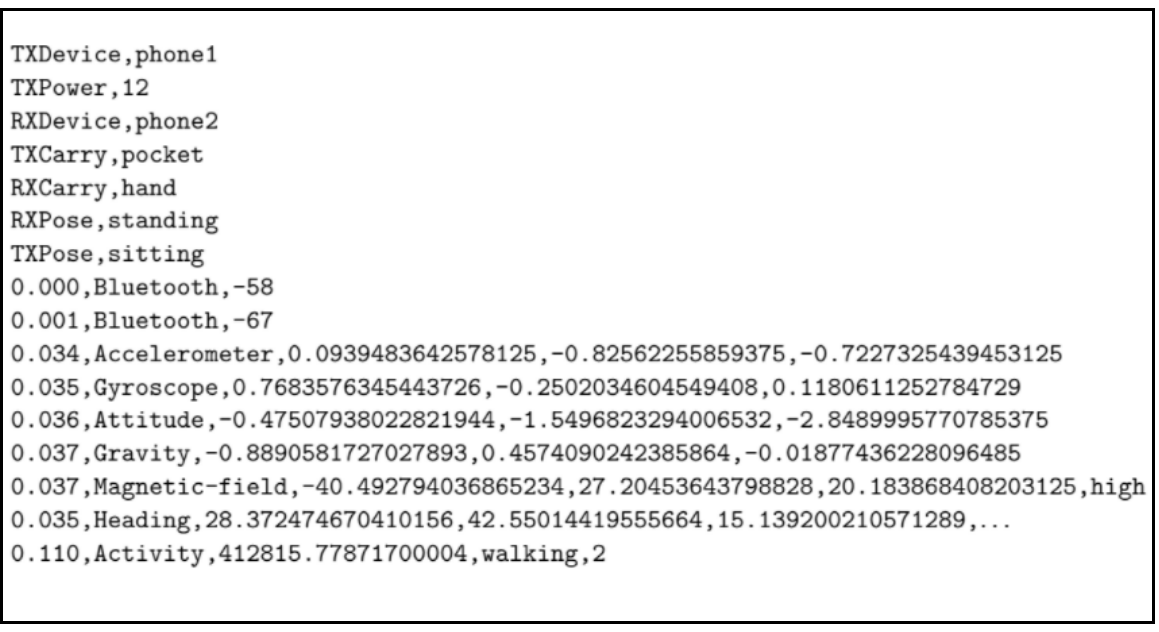
\includegraphics[width=0.5\textwidth]{img/data.png}
\caption[]{Example of a section of a contact event file}
\label{fig:fig_1}
\end{figure}
There were also accompanying meta data files providing additional information on events - the phone carriage state, step size (in seconds) for the 4s looks, distance in meters and the granularity of distance events (i.e., coarse-grain vs fine-grain).
Coarse  grain  events  differ  by  up  to  2.1  meters and fine  grain events differ by up to 0.9 meters.\cite{b1}  The distance label distributions of coarse grain and fine grain events can be seen in Table \ref{table:distance_label_dist}.\cite{b2} below.
\begin{table}[h!]
\begin{center}
\begin{tabular}{ c c c c c }
 Distance\_label & Fine\_Grain & Coarse\_Grain  \\ \hline
 1.2\_meters & 2563 & 0 \\ 
 1.8\_meters & 2569 & 2567  \\  
 3\_meters & 2553 & 0  \\
 4.5\_meters & 2556 & 2562 
\end{tabular}
\caption{Distance Label Distribution}
\label{table:distance_label_dist}
\end{center}
\end{table} 

Outputs of the models were submitted  through the NIST scoring software, and the performance of the model could be determined by evaluating the probability of miss and the probability of false alarm.

\begin{equation} \label{Pmiss}
{\mathbf{\textbf{Pmiss}} ={\frac{Num\ of\ ref = TC4TL\ and\ hyp = not - TC4TL}{ref = TC4TL}}}
\end{equation}

\begin{equation} \label{Pfa}
{\mathbf{\textbf{Pfa}} ={\frac{Num\ of\ ref = not-TC4TL\ and\ hyp = TC4TL}{ref = not-TC4TL}}}
\end{equation}

The two probabilities were then combined through the use of a normalised decision cost function (nDCF)

\begin{equation} \label{nDCF}
{\mathbf{\textbf{nDCF}} ={\frac{w_{miss} P_{miss} +w_{fa} P_{fa}}{min(w_{miss} , w_{fa})}}}
\end{equation}

where $w_{miss}$ and $w_{fa}$ are costs associated with missed and spurious detections. The challenge weights have been set by NIST: $w_{miss}$ = 1 and $w_{fa}$ = 1. \cite{b7} \cite{b8} 

\section{Related Work}
\begin{itemize}

\item Gomez et al\cite{b2}  used two ML models to estimate the distance between two phones. i)Multi-Layer Perceptron (MLP) - uses neural networks. With this approach, they were able to improve the previous model results by a significant margin, however, their error rate was not perfect.  ii) Gradient Boosting Machine (GBM) - it is a tree-based method. They chose it because of its good performance with tabular data. Both models were able to significantly reduce the average error in comparison to current methods. Future Work: GBM can be improved by investigating the following: Creating a normalized decision cost function metric for tuning and training, Performing analysis on the possibility of an interaction existing between the transmitter device and the RSSI values and having a Threshold analysis for weighting higher distance classes. For MLP, Explore the possibility of considering other sensor data such as accelerometer or gyroscope.

\item Hatke et al\cite{b8} proposed digital contact tracing to augment manual contact tracing using BLE signals between two phones. Their approach is to develop a TCFTL detector that uses a binary function that maps RSSI estimates into a yes or no decision regarding the too close portion of the detector. The detector performed roughly at 30% for detection of too close being true. There are still some hindrances that can be improved by an application of M and N detectors to provide robust performance.

\item He and Printz\cite{b9} proposed a 2-stage deep learning-based classifier for BLE proximity detection. Contributions: Use BLE RSSI histogram representation to reduce the multi-path effect. Introduce IMU data to compensate for the signal blocking from phone carriage states, leverage a deep learning-based classifier to model the impact of multi-path effect and phone carriage state on proximity detection. They say their model is both storage efficient and computationally efficient due to the 2-stage structure. They have verified their idea and got a very good result on the Too Close for Too Long (TC4TL) Challenge\\

\end{itemize}

 \section{Data Exploration and Analysis}
The MIT Matrix Data \cite{b6} and MITRE Range Angle \cite{b7} data sets were collected by the PACT (Private Automated Contact Tracing) Team at MIT. Both  data sets contain Bluetooth RSSI values collected under different environmental conditions (examples include room size, altitude, position angles, range and orientations). They also identify the types of phone used (iPhone X for example), and sensor data: along the RSSI values, we have accelerometer, gyroscope, gravity, altitude and activity readings – all these describing the pose, activity and environment in which the data was collected. While these 2 data sets contain similar features, their data is distinct in many ways: as an example, MITRE contains more devices than MIT Matrix Data, and this was taken into account to avoid discrepancies during training and testing phases.  The training set contains 15,552 csv files collected in different phone carriage states, the distance (1.2, 1.8, 3.0 or 4.5 meters) at which the csv file was collected, the step size determining the difference in seconds between the previous collected 4 seconds chirp and the next, and a binary categorical column determining if the csv file is coarse grained or not. This train set was collected from the MITRE Angled data set. While The development and test sets, collected from the MIT Matrix Data, have similar sensor attributes to the train set, these differ in the types of devices used and the distances measured in data collection. The high diversity of devices in the MITRE data was affecting performance on the test set in our project.\\


\section{Problem Formulation Considerations}

\begin{itemize}
\item x xxxxxx xxxxxxxxx xxx xxxx xxxx x xxx xxxx xxxx xxxxxxxxxxxx xxxx xxxxx x
\item x xxxxxx xxxxxxxxx xxx xxxx xxxx xxxxxx xxxxxxxxx xxx xxxx xxxx xxxxxxxxxxxx xxxx xxxxx x
\item x xxxxxx xxxxxxxxx xxx xxxx xxxx xxxxxxxx xxxx xxxxx x
\item x xxxxxx xxxxxxxxx xxx xxxx xxxxx xxxx xxxx xxxxx xxxx xxxxx x

\end{itemize}

\section{Strategy 1}
To create a baseline, we extracted features from the Bluetooth readings by averaging the RSSI values of each chirp. Then, we padded the missing values with zeros. Next, we used a random forest classifier to predict whether an interaction occurred within the specified distance. This approach had an average nDCF score of 0.6275 when evaluated against the dev set.\\


\section{Strategy 2}
We padded missing RSSI values with zeros, and concatenated both the MIT and MITRE datasets \cite{b6} \cite{b7} to include missing devices and distances, we obtained an Augmented set that took into account the missing devices and distances (1.0, 1.5, 2.0,2.5, 3.0, 3.5, 4.0, 4.5 meters) that were in the MITRE dataset, and then trained on a merged MITRE and MIT Matrix dataset – this was done to solve the discrepancies in evaluation results. With the merged MIT and MITRE datasets, we tested the environment as a feature, but this did not improve the performance of our model (no improvement on the nDCF).\\

\begin{table}[h!]
\begin{center}
\begin{tabular}{ c c c c c }
 Subset & D & P\_miss & P\_fa & nDCF  \\ \hline
 fine\_grain & 1.20 & 0.075 & 0.012 & 0.087 \\ 
 fine\_grain & 1.80 & 0.054 & 0.0186 & 0.073 \\  
 fine\_grain & 3.00 & 0.033 & 0.059 & 0.092 \\
 coarse\_grain & 1.80 & 0.086 & 0.022 & 0.108 \\ \hline
 total\_error & & 000 & 000 & \textbf{000}
\end{tabular}
\caption{Random Forest results}
\label{table:c_m3}
\end{center}
\end{table}

\section{Strategy 3}
xx xxxx xxxxxxxx xxxx xxxx xxxxx x xxxxxxxxx xxxxx xxx xxxxxxx xxxxxxxxxx xxxxxx xxxxxxxxx xxx xxxx xxxx xxxxxxxx xxxx xxxxxxxx x xxxxxxxxx xxxxx xxx xxxx xx\\

\begin{table}[h!]
\begin{center}
\begin{tabular}{ c c c c c }
 Subset & D & P\_miss & P\_fa & nDCF  \\ \hline
 fine\_grain & 1.20 & 0.075 & 0.012 & 0.087 \\ 
 fine\_grain & 1.80 & 0.054 & 0.0186 & 0.073 \\  
 fine\_grain & 3.00 & 0.033 & 0.059 & 0.092 \\
 coarse\_grain & 1.80 & 0.086 & 0.022 & 0.108 \\ \hline
 total\_error & & 000 & 000 & \textbf{000}
\end{tabular}
\caption{Other models results}
\label{table:other}
\end{center}
\end{table}

\section{Strategy 4}
xx xxxx xxxxxxxx xxxx xxxx xxxxx x xxxxxxxxx xxxxx xxx xxxxxxx xxxxxxxxxx xxxxxx xxxxxxxxx xxx xxxx xxxx xxxxxxxx xxxx xxxxxxxx x xxxxxxxxx xxxxx xxx xxxx xx\\
\begin{table} [!h]
\centering
\resizebox{0.45\textwidth}{!}{
    \begin{tabular}{p{2.8cm} | p{0.7cm} p{0.7cm}p{0.7cm}p{0.7cm}||p{1.0cm}}
    \textbf{} & Fine Grain 1.2m & Fine Grain 1.8m & Fine Grain 3.0m & Coarse Grain 1.8m & Average nDCF \\ 
    
    \hline
    RF (proposed) & \text{000} & \text{000} & \text{000} & \text{000} & \textbf{000} \\
   
     \hline
    Other (proposed) & \text{000} & \text{000} & \text{000} & \text{000} & \textbf{000} \\
    
    \hline
    GBM & \text{0.6} & \text{0.52} & \text{0.58} & \text{0.37} & \text{0.5175} \\
    
    \hline
    MLP & \text{0.61} & \text{0.48} & \text{0.55} & \text{0.44} & \text{0.52} \\
    
    \hline
    Contact-Tracing-Project & \text{0.68} & \text{0.54} & \text{0.59} & \text{0.41} & \text{0.555} \\
    
    \hline
    LCD  & \text{0.6} & \text{0.58} & \text{0.63} & \text{0.55} & \text{0.59} \\
    
    \end{tabular}}
    \caption{ Results compared to state of the art}
\label{table:results}
\end{table}

\section{Discussion}
The results obtained with our proposed models are shown in table \ref{table:results}, along with results from current state-of-the-art methods. The table shows that ............ significantly reduce the average error in comparison to current state-of-the-art methods. 



\section{Future Work}

\begin{itemize}
\item x xxxxxx xxxxxxxxx xxx xxxx xxxx xxxxxxxxxxxx xxxx  xxxx xxxx xxxxxxxxxxxx xxxx xxxxx x
\item x xxxxxx xxxxxxxxx xxx xxxx xxxx xxxxxxxxxxxx xxxx xxxxxxxxxxxx xxxx xxxxx x
\item x xxxxxx xxxxxxxxx xxx xxxx xxxx xxxxxxxxxxxx xxxx xxxxx xxxxxxxxx xxx xxxx xxxx xxxxxxxxxxxx xxxx xxxxx x
\item x xxxxxx xxxxxxxxx xxx xxxx xxxx xxxxxxxxxxxx xxxx x xxxxx xxxxxxxxx xxx xxxx xxxx xxxxxxxxxxxx xxxx xxxxx x

\end{itemize}
\section{Some Additional Considerations}
 A context-specific approach should be adopted. Some of the considerations that may relate to an Irish context are outlined below: 

\begin{itemize}
\item {\emph{Users of a Contact Tracing App}} \cite{b3}
1) data and public trust (how is the general users made aware of who is collecting the data, for what purpose and who manages it (i.e. accountability; user agreements); 2) the ability for users to opt-in or opt-out of the process (make the app mandatory or voluntary/participatory); 3) accessibility of source code (public availability of source code and other material); 4) reproducibility and consistent results; 5) an assessment of whether the data and other development material will be shut down when Covid-19 fazes out and there is no need for contact tracing.

\item {\emph{Ethics of Contact Tracing Apps}}\cite{b3}
In their 2020 paper, Parker et al set out
a number of ethical considerations that relate to the use of mobile phone apps to enable rapid contact tracing. They argue: 1) The ethical assessment should be analysed against the scale of the deaths and suffering; 2) The justification of blanket lockdowns would be weaker were it possible to manage physical distancing in a more evidence-based, risk-adjusted way. 3) There are privacy concerns relating to data collection scope and duration; 4) An app has the potential to be autonomy enhancing e.g. allowing people to make informed choices. 5) The use of incentives could adversely impact those who do not have access to suitable smart-phones. 6) An app could provide a way for professionals and institutions to meet their obligations 
\item {\emph{AI must be Trustworthy}}\cite{b3}
In 2019 a set of Ethics Guidelines for Trustworthy AI were developed on behalf of the European Commission. They devised a non-exhaustive list of requirements for trustworthy AI that include systemic, individual and societal aspects. In summary, they are: 
1) Human agency and oversight;
2) Technical robustness and safety; 
3) Privacy and data governance; 4) Transparency; 
5) Diversity, non-discrimination and fairness;
6) Societal and environmental wellbeing;
7) Accountability 
\item {\emph{A National AI Strategy for Ireland.}}\cite{b3}
This document published in July 2021 holds three core principles: 1) adopting a human-centric approach to application of AI; 2) staying open and adaptable to new innovations; and 3) ensuring good governance to build trust and confidence for innovation to flourish. 
\item {\emph{The European Commission’s Coordinated Plan on AI: 2021 Review.}}\cite{b4}
In order to create EU global leadership on trustworthy AI, a set of joint actions for the European Commission and Member States was identified: 1) set enabling conditions for AI development and uptake in the EU; 2) make the EU the place where excellence thrives from the lab to the market; 3) ensure that AI works for people and is a force for good in society; and 4) build strategic leadership in high-impact sectors.
\item {\emph{Bad Actor Attacks on Contact Tracing Apps.}}\cite{b5}
The Trinity College Dublin funded “Testing Apps for COVID-19 Tracing” (TACT) project, highlights the issue of false positive proximity warnings, so as to disconcert people or to discredit the system. They believe that : 1) preventing the attack could add significant complexity to the overall system and might not be feasible; 2) that the impact of the attack increases as more people run the tracing app, and 3) that the attack can be targeted against key staff in some scenarios so that targeting even with a small amplification factor may cause noticeable damage.
\item {\emph{Pre-Testing with the Public.}}\cite{b6}
In their report on Ireland’s contact-tracing app COVID Tracker, Julienne et al (2020) identify the value of pre-testing contact-tracing apps. They contend it boosts uptake, trust and participation. 
\item {\emph{A Potentially Misleading API.}}\cite{b7}
A 2021 report by Leith et al identified that while many health authorities have committed to making the code for their contact tracing apps open source, they depend upon the non open source Google/Apple Exposure Notification (GAEN) API for their operation. This has limited public documentation, and uses a filtered Bluetooth LE signal strength measurement that can be potentially misleading with regard to the proximity between two handsets.


\end{itemize}



\section*{Acknowledgment}
This publication has emanated from research conducted with the financial
support of Science Foundation Ireland under Grant number 18/CRT/6183. For the purpose
of Open Access, the author has applied a CC BY public copyright licence to any
Author Accepted Manuscript version arising from this submission.\\
We would also like to acknowledge Mayug Maniparambil for mentoring us throughout the project; and Omid Sadjadi, for providing us with information about the data.

\begin{thebibliography}{00}
\bibitem{b1}Nist.gov. 2020. NIST Pilot Too Close For Too Long (TC4TL) Challenge Evaluation Plan. [online] Available at: <https://www.nist.gov/system/files/documents/2020/07/01/2020 NISTPilot TC4TL Challenge Evaluation Plan v1p3.pdf> [Accessed 02 November 2021].
\bibitem{b2}Docs.h2o.ai. 2020. Categorical\_Encoding — H2O 3.32.0.2 Documentation. [online] Available at: <http://docs.h2o.ai/h2o/latest-stable/h2o-docs/data-science/algo-params/categorical\_encoding.html> [Accessed 03 November 2021].
\bibitem{b3} Hatke, G.F., Montanari, M., Appadwedula, S., Wentz, M., Meklenburg, J., Ivers, L., Watson, J. and Fiore, P., 2020. Using Bluetooth Low Energy (BLE) signal strength estimation to facilitate contact tracing for COVID-19. arXiv preprint arXiv:2006.15711. https://arxiv.org/abs/2006.15711 
\bibitem{b4}reference details to be added here [online] Available at: <https://digital-strategy.ec.europa.eu/en/library/coordinated-plan-artificial-intelligence-2021-review> [Accessed 03 November 2021].
\bibitem{b5} Farrell, S. and Leith, D.,2020. A Coronavirus Contact Tracing App Replay Attack with Estimated Amplification Factors 
\bibitem{b6}Julienne, H., Lavin, C., Belton, C., Barjaková, M., Timmons, S. and Lunn, P.D., 2020. Behavioural pre-testing of COVID Tracker, Ireland’s contact-tracing app. [online] Available at: <to do> [Accessed 03 November 2021].
\bibitem{b7}Leith, D.J. and Farrell, S., 2021. Google/Apple exposure notification due diligence. In Proceedings of the CoronaDef Workshop, Network and Distributed System Security Symposium (NDSS). [online] Available at: <to do> [Accessed 03 November 2021].
\bibitem{b8}Gasser U, Ienca M, Scheibner J, Sleigh J, Vayena E. Digital tools against COVID-19: taxonomy, ethical challenges, and navigation aid. Lancet Digit Health. 2020 Aug;2(8):e425-e434. doi: 10.1016/S2589-7500(20)30137-0. Epub 2020 Jun 29. PMID: 32835200; PMCID: PMC7324107.
\bibitem{b9}Pagliari C. The ethics and value of contact tracing apps: International insights and implications for Scotland's COVID-19 response. J Glob Health. 2020 Dec;10(2):020103. doi: 10.7189/jogh.10.020103. PMID: 33110502; PMCID: PMC7510337.
\bibitem{b10}Vinuesa(2020).
\bibitem{b11}AI, H., 2019. High-level expert group on artificial intelligence. Ethics guidelines for trustworthy AI https://digital-strategy.ec.europa.eu/en/library/ethics-guidelines-trustworthy-ai 
\bibitem{b12} Stephens, M., Cala, G., Greene, K., Keenan, K.E., Robinson, A., Shi, L., Ufford, D. and Valdez, Z., 2021. Workshop Report: Challenges for Digital Proximity Detection in Pandemics: Privacy, Accuracy, and Impact. https://nvlpubs.nist.gov/nistpubs/SpecialPublications/NIST.SP.1268.pdf
\bibitem{b13}MITRE Range Angle Structured Data set [online] Available at: <https://github.com/mkrangle/MITRE-Range-Angle-Structured> [Accessed 17 November 2021].
\bibitem{b14}MIT Matrix Data [online] Available at: <https://github.com/mitll/MIT-Matrix-Data> [Accessed 17 November 2021].
\bibitem{b15}Digital Communications Lab - Team: LCD, 2020. Contactar. https://tc4tlchallenge.nist.gov
\bibitem{b16}He, T., Printz, M. and Chan, G., 2020. TC4TL Challenge: A 2-Stage Classifier For Proximity Detection With BLE And IMU. https://tc4tlchallenge.nist.gov

\end{thebibliography}


\end{document}
